\documentclass{beamer}

\usepackage{lipsum}      % Use for dummy text, for instance \lipsum[1-4] prints 4 paragraphs

\mode<presentation>{\usetheme{Ringerike}}
\usepackage[english]{babel}
\usepackage[latin1]{inputenc}
\usepackage{caption}
\usepackage[normalem]{ulem}
\usepackage{multicol}
\usepackage{vwcol}
\usepackage{multirow}
\usepackage{tabularx}
\usepackage{subfig}
\usepackage{makecell}
\newcolumntype{C}{>{\centering\arraybackslash}X}
\newcolumntype{Y}{<{\centering\arraybackslash}Y}

%\usepackage{amsmath,amsthm, amssymb, latexsym}
%\boldmath

% Size of poster
\usepackage[size=a0,orientation=portrait]{beamerposter}

\addtobeamertemplate{block begin}{}{\setlength{\parskip}{30pt plus 1pt minus 1pt}}
\setbeamertemplate{caption}[numbered]

% Bibliography colors and labels
\setbeamertemplate{bibliography item}{\color{white}\insertbiblabel}
\setbeamercolor{bibliography entry item}{fg=white}
\setbeamercolor{bibliography entry author}{fg=white}
\setbeamercolor{bibliography entry title}{fg=white} 
\setbeamercolor{bibliography entry location}{fg=white} 
\setbeamercolor{bibliography entry note}{fg=white}

\title{First results from the new station NYALE13S}
%\subtitle{A New Software for Geodetic Analysis}
\author{Ann-Silje Kirkvik, Michael D\"ahnn, Ingrid Fausk}
\newcommand{\contact}{ann-silje.kirkvik@kartverket.no}
\institute{Norwegian Mapping Authority, Geodetic Institute}
\date{March 14th-18th, 2021}

\usebackgroundtemplate{
\includegraphics[width=\paperwidth]{figure/earth}}

\begin{document}
\begin{frame}[t]
  % Top title area
  \color{white} 
  \vspace*{2cm}
  \begin{columns}
    \begin{column}[t]{.97\textwidth}
      {\bfseries\fontsize{88}{120}\selectfont \inserttitle}
      %{\fontsize{88}{120}\selectfont\kern2cm---\kern2cm\insertsubtitle}
    \end{column}
  \end{columns}

  \vspace*{2cm}
  \begin{columns}
    \begin{column}[t]{.25\textwidth}
      {\fontsize{30}{36}\selectfont\insertauthor\\[0.5cm]
        \fontsize{30}{36}\selectfont{\itshape\insertinstitute}\\
        \fontsize{24}{18}\selectfont\texttt{\contact}}
    \end{column}

    \begin{column}[t]{.7\textwidth}
      {\fontsize{30}{36}\selectfont\setlength{\parskip}{30pt}At the Norwegian Mapping Authority, we are currently developing Where, a new
software for geodetic analysis. Where is built on our experiences with the
Geosat software, and will be able to analyse and combine data from VLBI, SLR,
GNSS and DORIS. The software is mainly written in Python which has proved very
fruitful. The code is quick to write and the architecture is easily extendable
and maintainable, while at the same time taking advantage of well-tested libraries
like the SOFA and IERS packages.

At the moment the VLBI analysis is close to ready. Comparison to other softwares
show that theoretical delay computations in Where are consistent with those. SLR
and GNSS analysis is well under way.

\vspace*{-10cm}

\endinput
}
      \raisebox{0cm}{\kern52.5cm\color{white}\tiny PHOTO: GETTY IMAGES}
    \end{column}
  \end{columns}

  \begin{columns}

    % Text area
    \begin{column}[t]{.48\textwidth}
      \begin{block}{Data}
        \begin{multicols}{2}
          % Why these sessions
On the 17th of February 2020 the new station NYALE13S observed its first
successful 24 hour session. The week before some data was successfully correlated,
but since it was only 88 observations spanning 3 hours the station was not included 
in the official database. There is still only a limited number of sessions available 
with observations from both NYALE13S (Ns) and NYALES20 (Ny). The few sessions that 
exist are used in this analysis and are listed in table \ref{tab:sessions}.

NYALE13S observed with a warm receiver until R1945. But the SEFD values used in the schedule was not
updated to reflect the cold receiver until R1947. At the same time the receiver
at NYALES20 started to heat up and observed with a warm receiver for the
remaining sessions. NYALE13S has been scheduled as a tag-along
station for all these sessions. NYALE13S used a DBBC3 and FlexBuff system. In
the end the DBBC3 malfunctioned and had to be sent for repairs. The DBBC3 was
later replaced with a new DBBC2, but by then the elevation encoder at NYALES20
had malfunctioned and also had to be sent for repairs.

\begin{table}
\captionsetup{labelfont={color=kvlightgreen}}
	\begin{tabularx}{\columnwidth}{X|X}
	Session & Date \\
	\hline
	R1934 & 2020 02 17 \\
	R1935 & 2020 02 24 \\
	R1936 & 2020 03 02 \\
	R1937 & 2020 03 09 \\
	\sout{R1938} & \sout{2020 03 16} \\
	R1939 & 2020 03 23 \\
	R1940 & 2020 03 30 \\
	\sout{R1941} & \sout{2020 04 06} \\
	\sout{R1942} & \sout{2020 04 14} \\
	\sout{R1943} & \sout{2020 04 20} \\
	R1944 & 2020 04 27 \\
	R1945 & 2020 05 04 \\
	R1946 & 2020 05 11 \\
	R1947 & 2020 05 18 \\
	R1948 & 2020 05 26 \\
	R1949 & 2020 06 02 \\
	\sout{R1950} & \sout{2020 06 08} \\
	R1951 & 2020 06 15 \\
	R1952 & 2020 06 22 \\
	\hline
	\end{tabularx}
\caption{\textcolor{white}{Sessions used in analysis. The struck through rows are sessions with no useful
 data from NYALE13S.}}
\label{tab:sessions}
\end{table}

\endinput

        \end{multicols}
      \end{block}
      
      \begin{block}{Analysis}
          Multiple solutions were tested to see how the parameterization might affect the final results. The number of observations
available from NYALE13S is very limited and the quality is for the most part poor due to the warm receiver and other
problems with the sessions. This lowers the degrees of freedom and increases the uncertainty in the estimates. Different
setups for troposphere parameterizations and fixing the celestial reference frame have been tested.

The analysis has been done using \textbf{Where} \cite{hjelle2018}. The default solution is the same which is used for 
regular R1 and R4 processing. This means all station and source coordinates, EOPs, clocks and troposphere are estimated, 
for more information see \cite{kirkvik2017b} and \cite{kirkvik2019}. The results are summarized in table 
\ref{tab:solutions} and selected plots from the two extremes in terms of estimated parameters (solution 0 and solution 9) 
are shown in figure \ref{fig:plots}. A priori coordinates for NYALE13S used in the analysis are computed based on the local 
tie vector since the coordinates in the original database is off by almost a meter. The baseline length and repeatability is 
calculated according to \cite{hofmeister2016}.
 

\begin{table}
\captionsetup{labelfont={color=kvlightgreen}}
	\begin{tabularx}{\columnwidth}{l|l|C|C|C}
	~\#~ & ~Setup~ & WBL & WBLR & dL \\
	\hline
	~0~ & ~\makecell[tl]{Default}~ & 1539.1932 [m] & 0.0032 [m] & 0.0001 [m] \\
	~1~ & ~\makecell[tl]{Troposphere gradients fixed (Ns)}~ & 1539.1943 [m] & 0.0026 [m] & 0.0012 [m] \\
	~2~ & ~\makecell[tl]{Troposphere gradients fixed (Ns and Ny) \\ 
	Zenith wet delay fixed (Ns and Ny)}~ & 1539.1936 [m] & 0.0025 [m] & 0.0005 [m] \\
	~3~ & ~\makecell[tl]{Troposphere gradients fixed (Ns) \\ 
	Two hour zenith wet delay (Ns)}~ & 1539.1936 [m] & 0.0025 [m]  & 0.0010 [m] \\
	~4~ & ~\makecell[tl]{Troposphere gradients fixed (Ns and Ny) \\ 
	Two hour zenith wet delay (Ns and Ny)}~ & 1539.1931 [m] & 0.0021 [m] & 0.0000 [m] \\
	~5~ & ~\makecell[tl]{Radio sources fixed}~ & 1539.1939 [m] & 0.0021 [m] & 0.0008 [m] \\
	~6~ & ~\makecell[tl]{Radio sources fixed \\ 
	Troposphere gradients fixed (Ns)}~ & 1539.1945 [m] & 0.0025 [m] & 0.0014 [m] \\
	~7~ & ~\makecell[tl]{Radio sources fixed \\ 
	Troposphere gradients fixed (Ns and Ny) \\ 
	Zenith wet delay fixed (Ns and Ny)}~  & 1539.1936 [m] & 0.0027 [m] & 0.0005 [m] \\
	~8~ & ~\makecell[tl]{Radio sources fixed \\ 
	Troposphere gradients fixed (Ns) \\ 
	Two hour zenith wet delay (Ns)}~ & 1539.1943 [m] & 0.0022 [m] & 0.0012 [m] \\
	~9~ & ~\makecell[tl]{Radio sources fixed \\ 
	Troposphere gradients fixed (Ns and Ny) \\ 
	Two hour zenith wet delay (Ns and Ny)}~ & 1539.1943 [m] & 0.0022 [m] & 0.0000 [m] \\
	\hline
	\end{tabularx}
\caption{\textcolor{white}{Weighted baseline length (WBL), weighted baseline length repeatability (WBLR) and difference 
between weighted baseline length and local tie vector (dL) for the different solutions. The second column described how 
a solution differs from the default solution.
}}
\label{tab:solutions}
\end{table}

\endinput

      \end{block}
    
      \begin{block}{Conclusions}
        \begin{multicols}{2}
          The length of the baseline 
vector is approximately 1.5km and there is a height difference between the stations of approximately
33 meters. In addition, the NYALE13S is very close to the coast. Are these stations close
enough to experience the same troposphere? The baseline length seem to agree better with the local tie
vector if the troposphere is treated the same at both stations. But the repeatability is too poor and
the number of sessions are too few to be really sure. The uncertainty is mostly due to the perfomance of 
NYALE13S. The local tie vector is also just a premilinary 
result without known uncertainties at the moment. There are GNSS stations close to both NYALE13S and
NYALES20. Troposphere estimates from these stations should be investigated to compare the troposphere
at the two locations.  
 
Regardless, the local tie computations need to be finalized and more and better observations are needed
from the VLBI antennas. Only two sessions have good quality (R1947 and R1952) and the weighted baseline
length repeatability would be significantly better if more sessions were of this quality. The repairs at
NYALES20 are imminent and hopefully more sessions with both stations can be recorded very soon.

\endinput

        \end{multicols}
      \end{block}
      
    \end{column}

    \begin{column}[t]{.48\textwidth}
      \begin{figure}
    % Number of observations NYALE13S
	\subfloat[\textcolor{black}{Number of observations - NYALE13S - Solution 0}.\label{fig:num-Ns-0}]
      {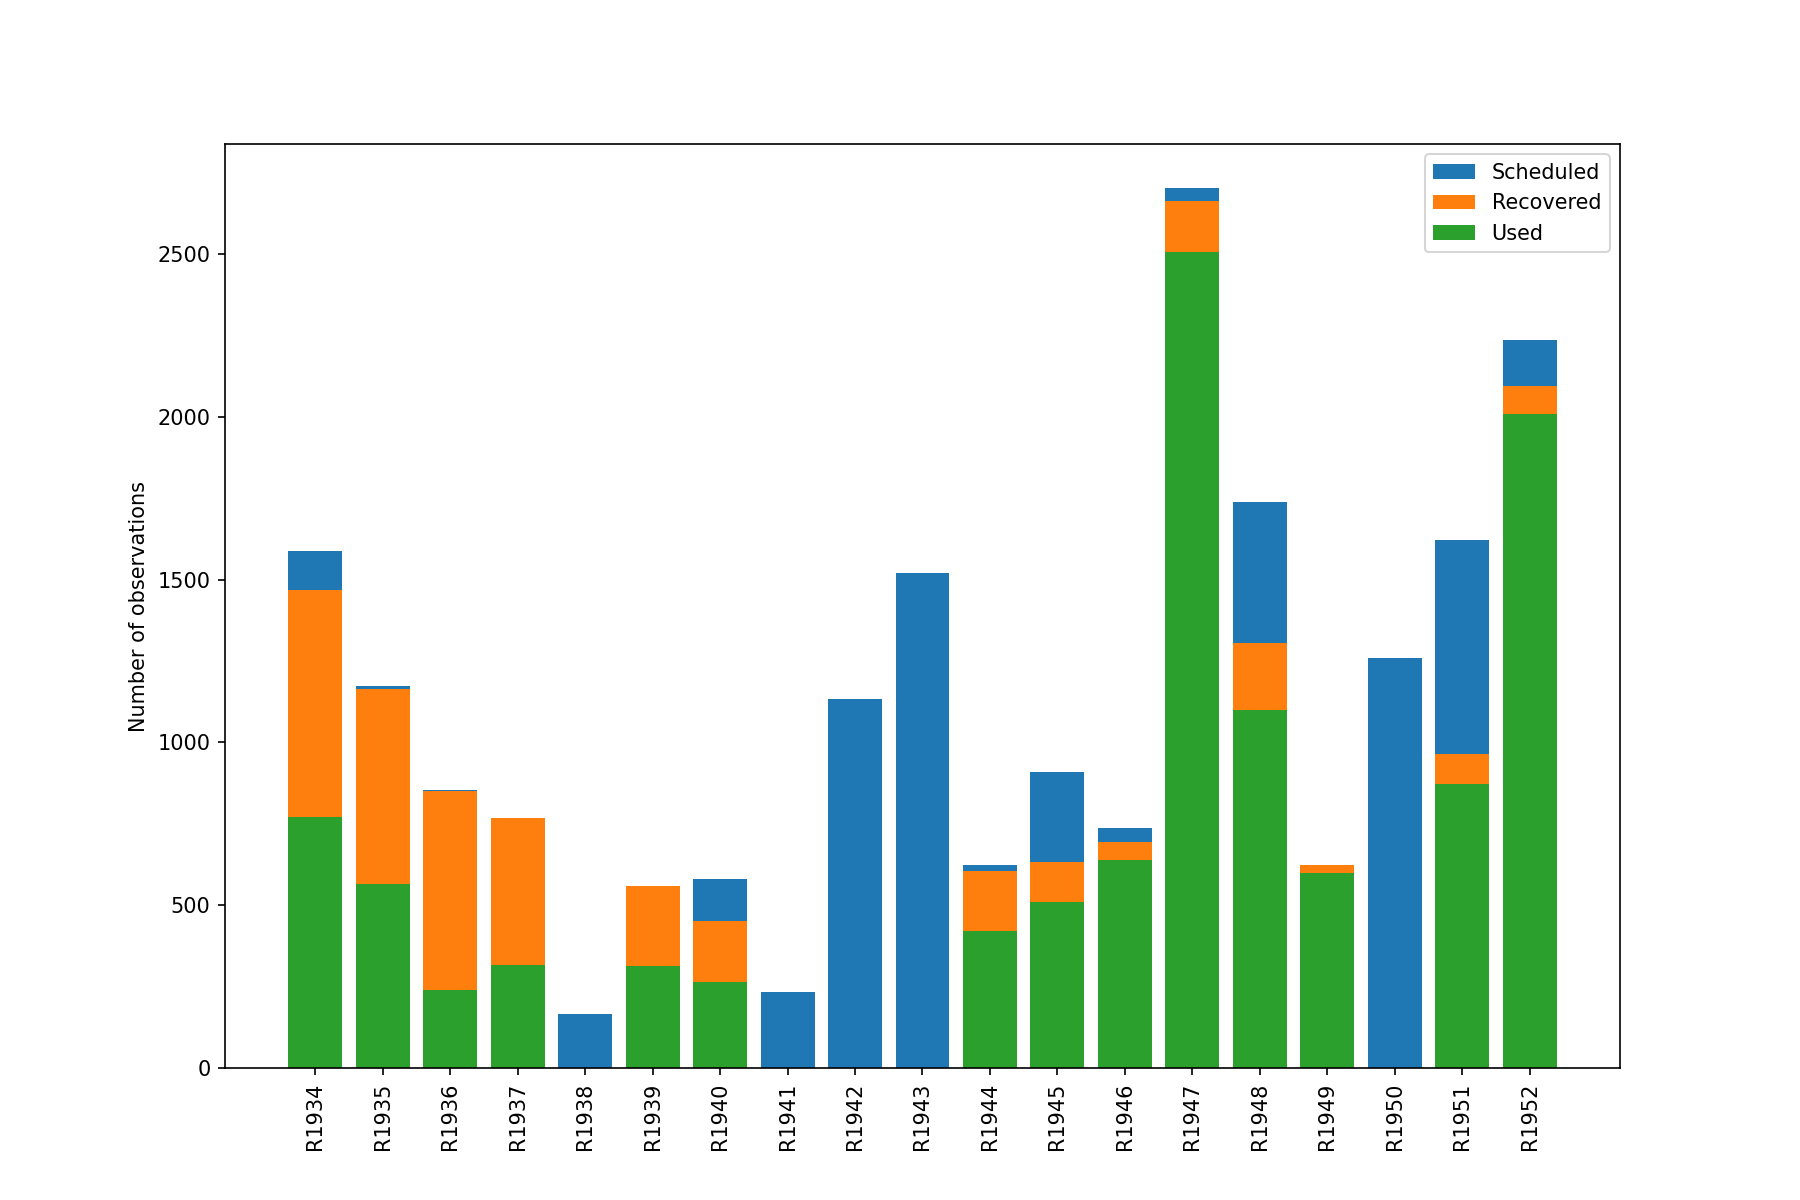
\includegraphics[width=0.5\linewidth]{figure/Num_obs_NYALE13S_nyale13s0}}
	\subfloat[\textcolor{black}{Number of observations - NYALE13S - Solution 9}.\label{fig:num_Ns-9}]
      {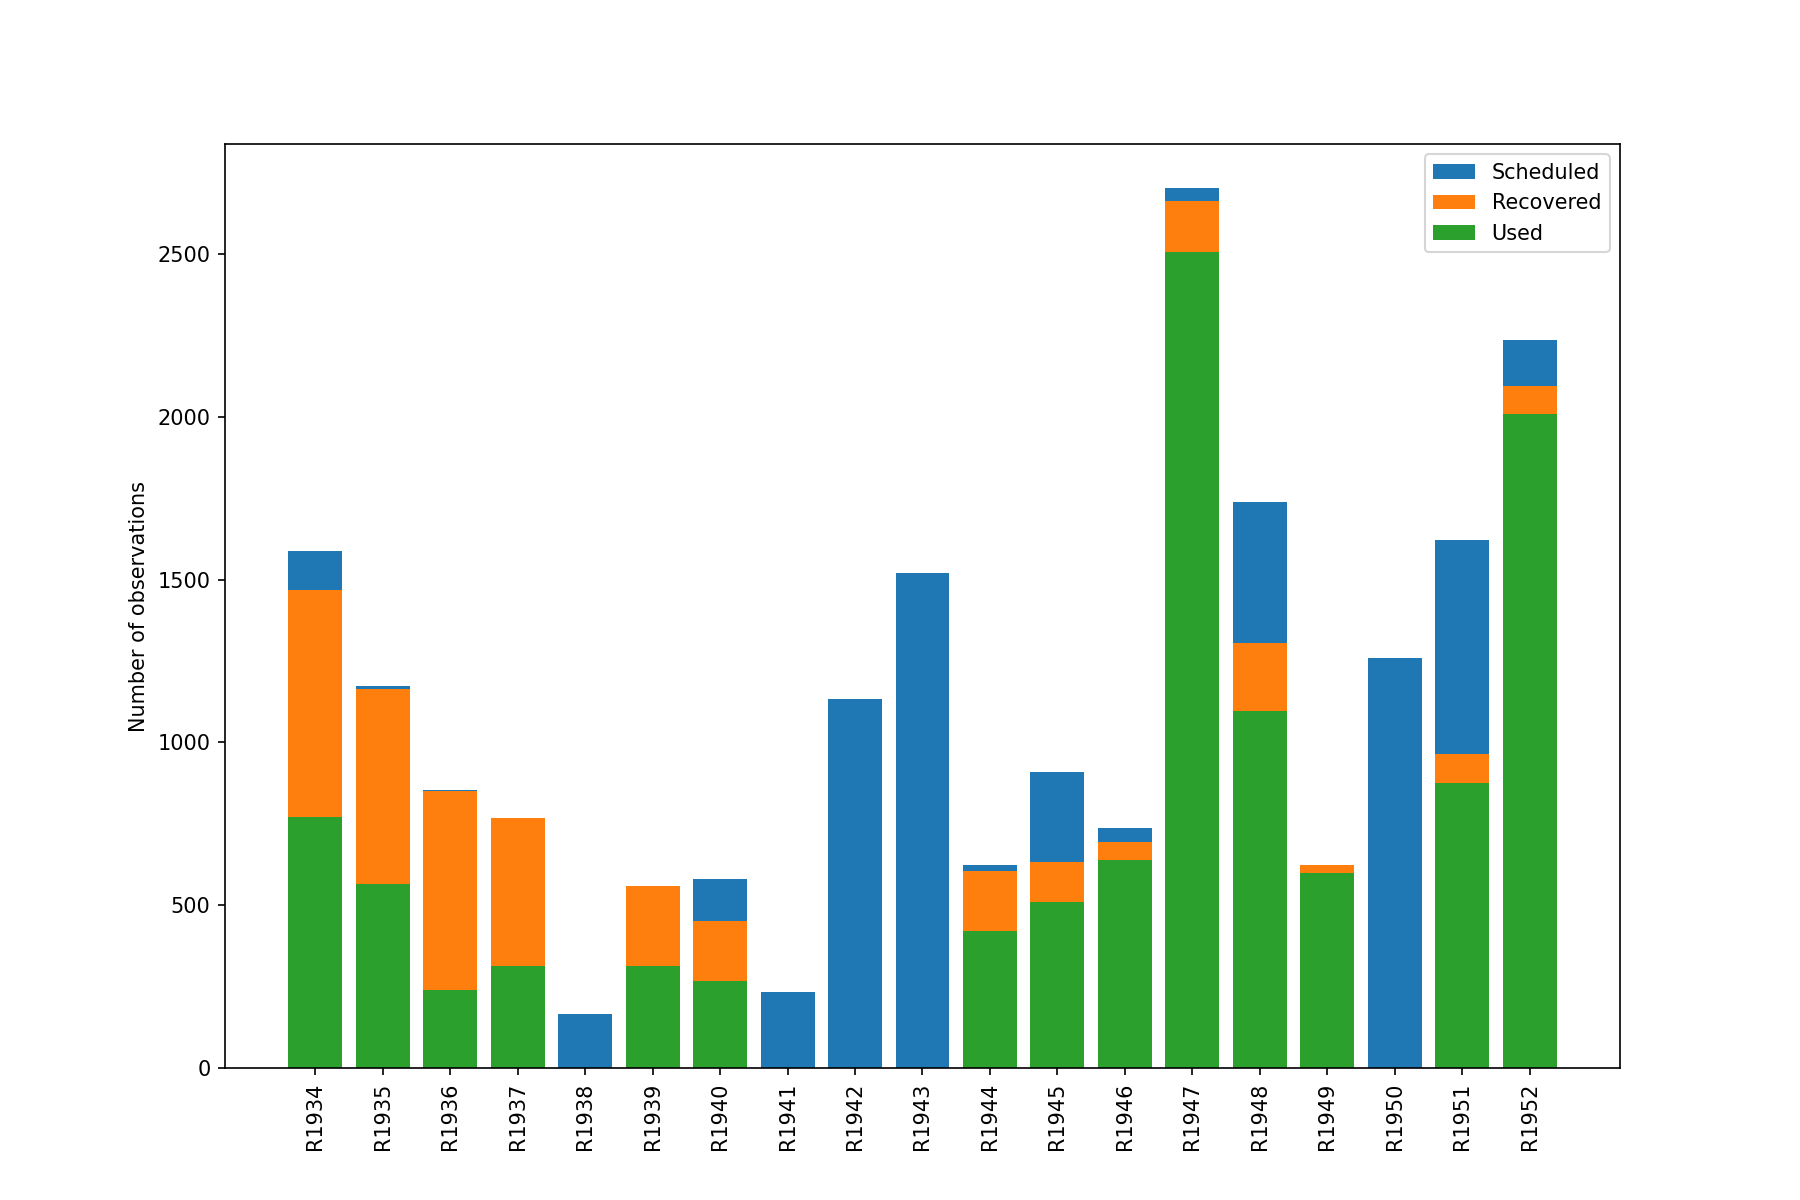
\includegraphics[width=0.5\linewidth]{figure/Num_obs_NYALE13S_nyale13s9}} \\
    % Number of observations NYALES20
	\subfloat[\textcolor{black}{Number of observations - NYALES20 - Solution 0}.\label{fig:num-Ny-0}]
      {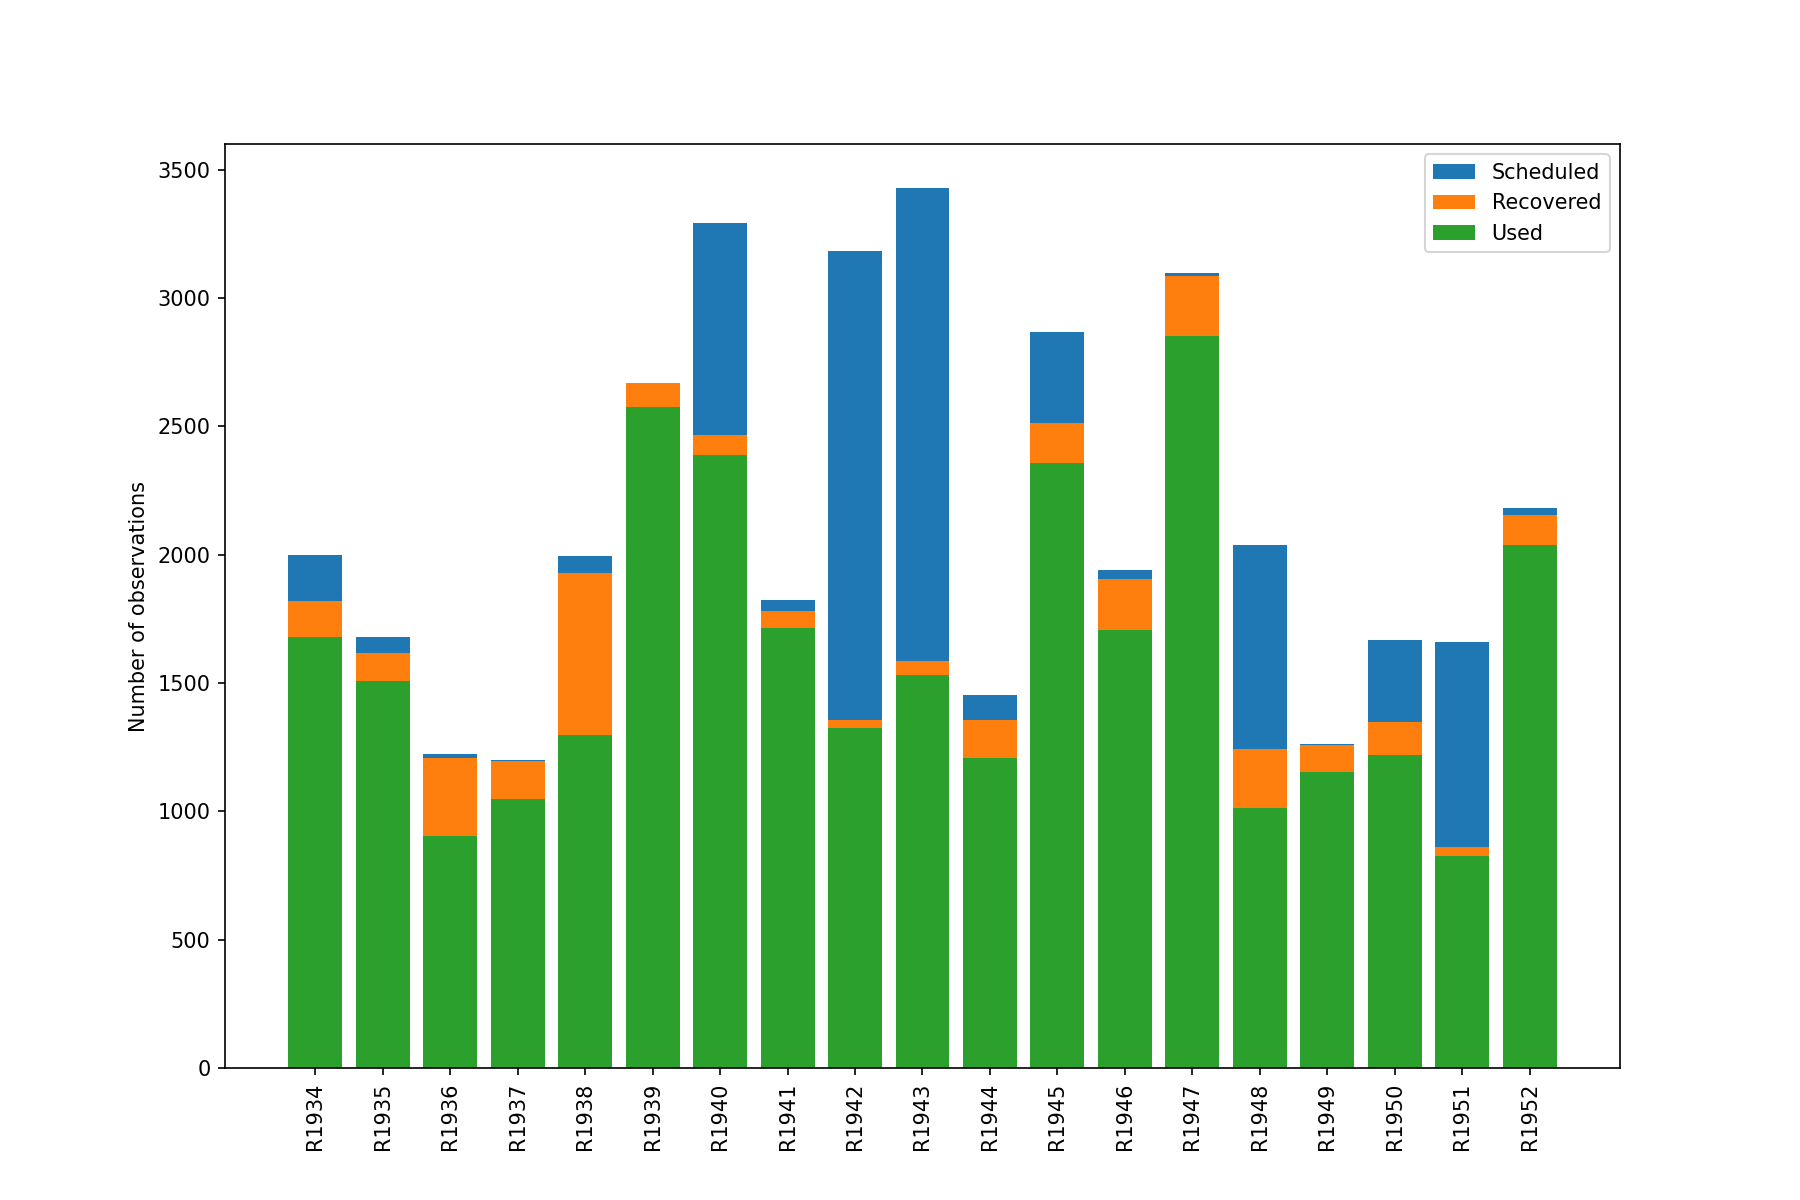
\includegraphics[width=0.5\linewidth]{figure/Num_obs_NYALES20_nyale13s0}}
	\subfloat[\textcolor{black}{Number of observations - NYALES20 - Solution 9}.\label{fig:num_Ny-9}]
      {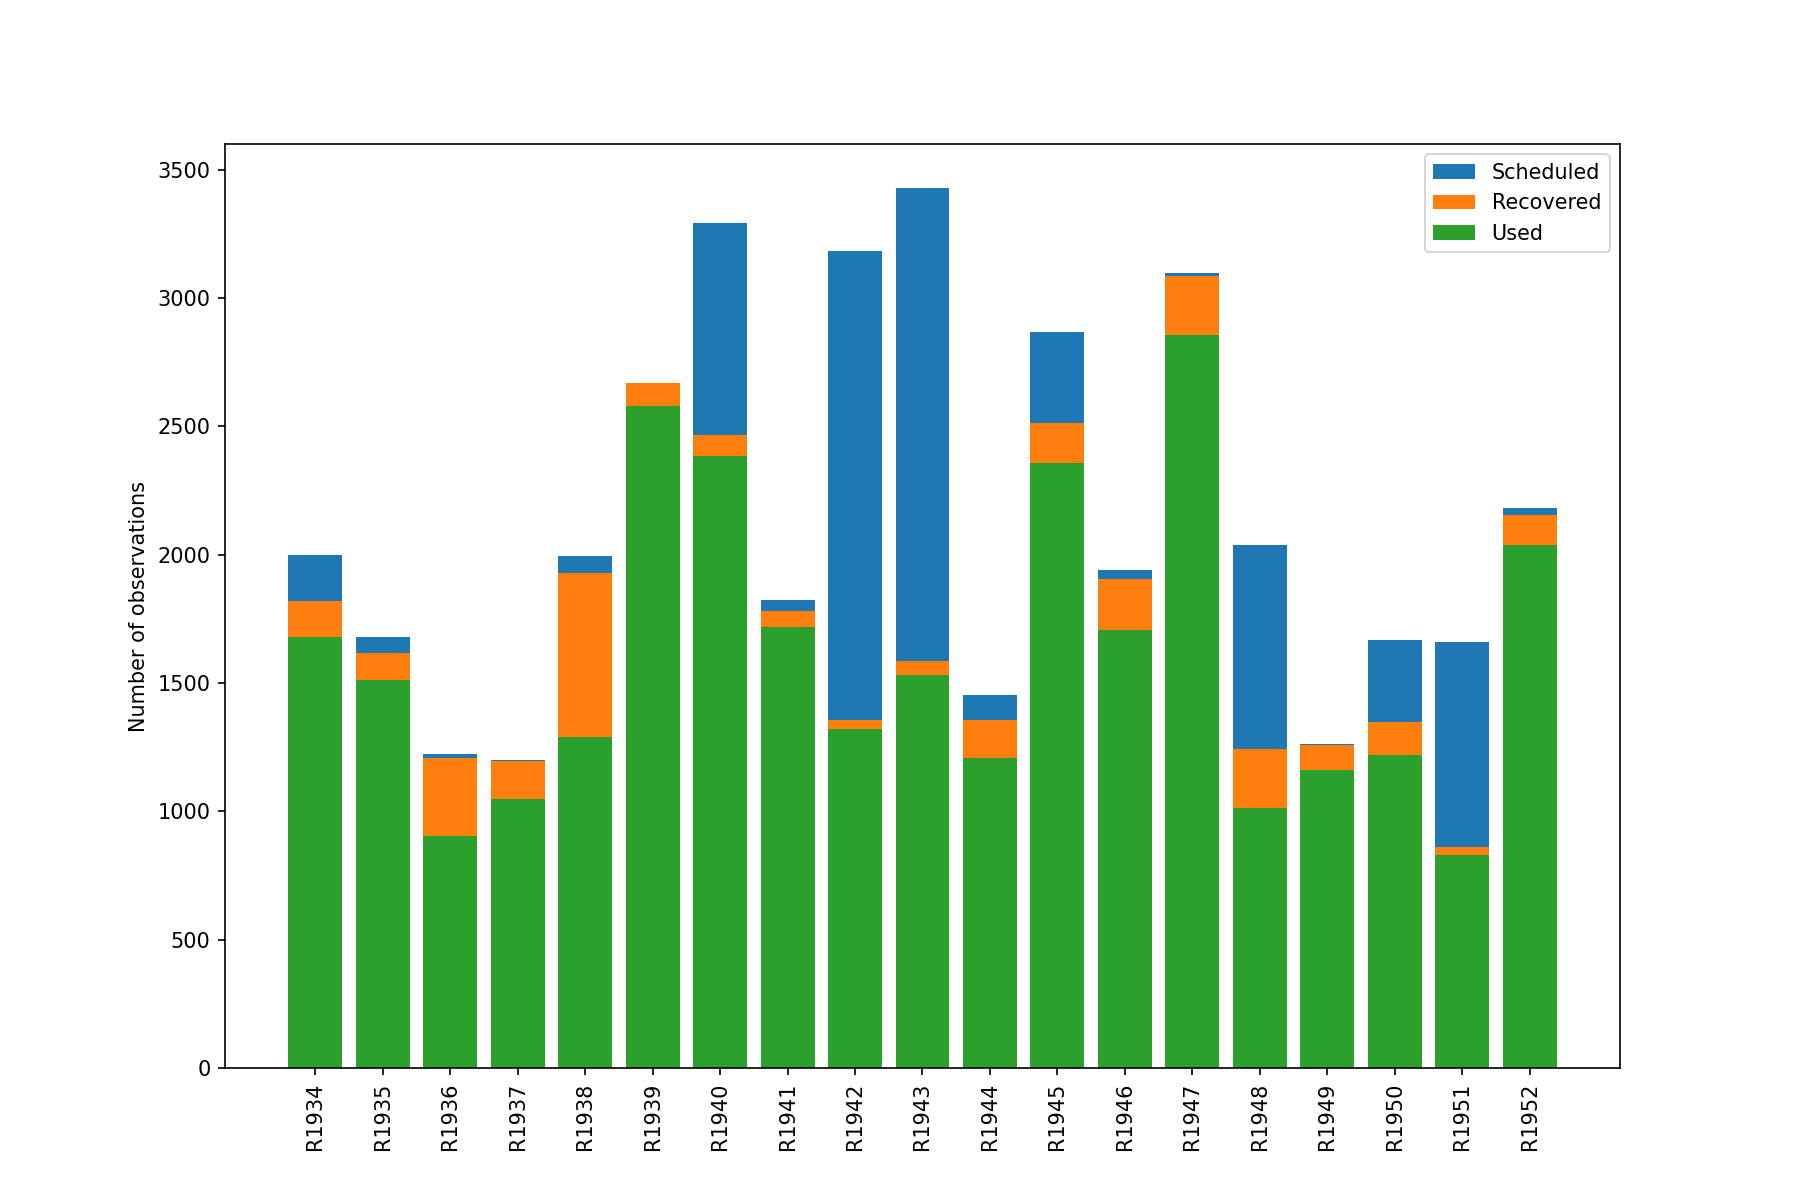
\includegraphics[width=0.5\linewidth]{figure/Num_obs_NYALES20_nyale13s9}} \\
    % Baseline lengths
	\subfloat[\textcolor{black}{Baseline length - NYALE13S/NYALES20 - Solution 0}.\label{fig:bl-0}]
      {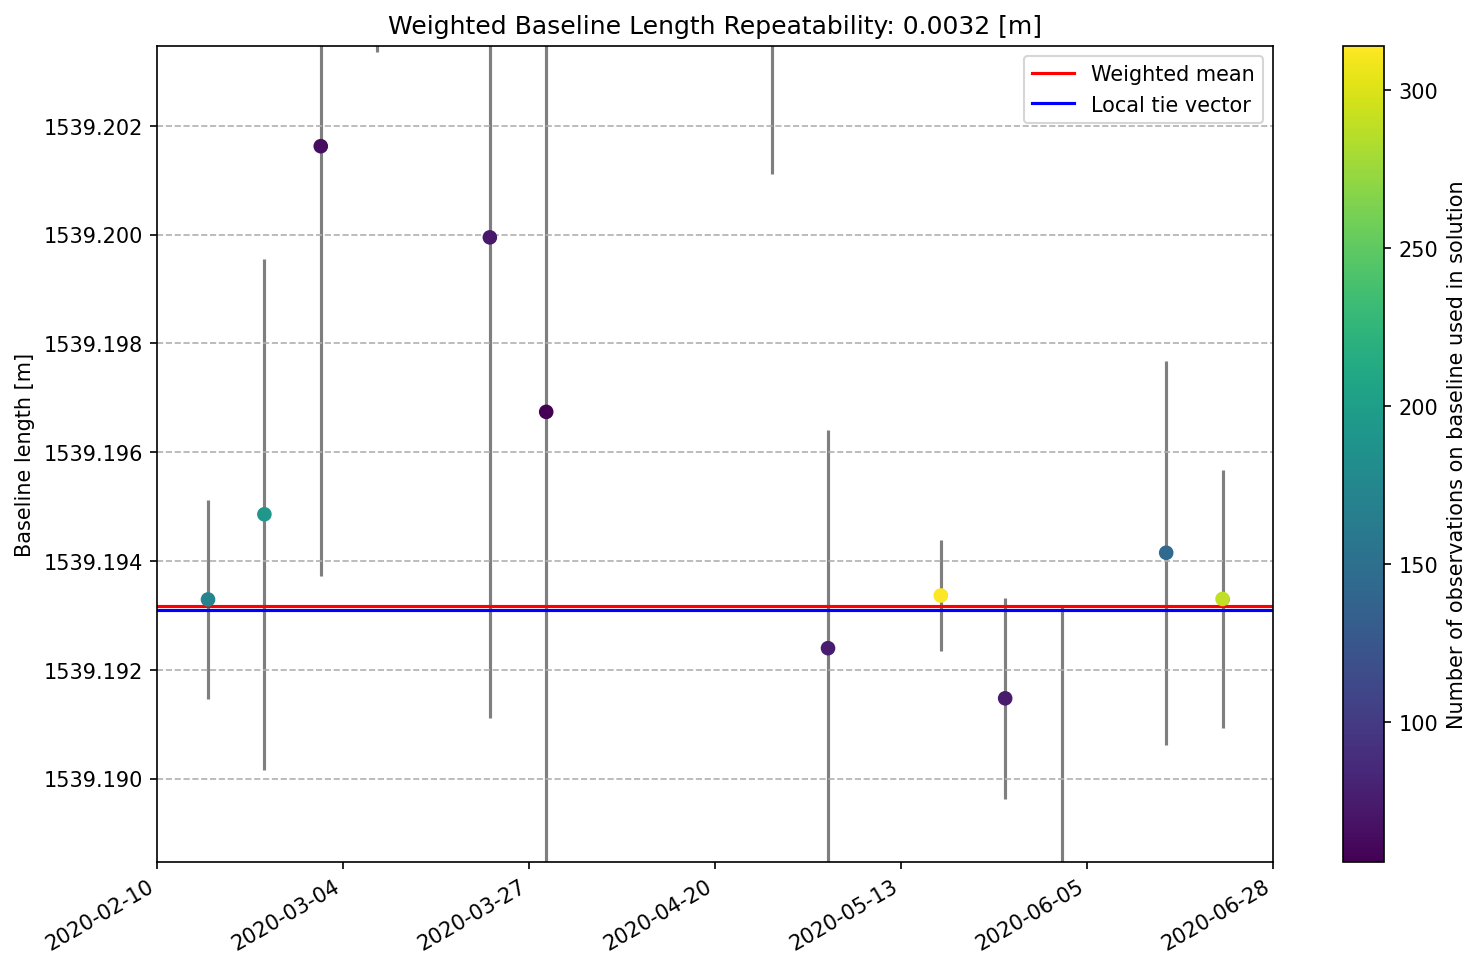
\includegraphics[width=0.5\linewidth]{figure/Baseline_NYALES20_NYALE13S_nyale13s0}}
	\subfloat[\textcolor{black}{Baseline length - NYALE13S/NYALES20 - Solution 9}.\label{fig:bl-9}]
      {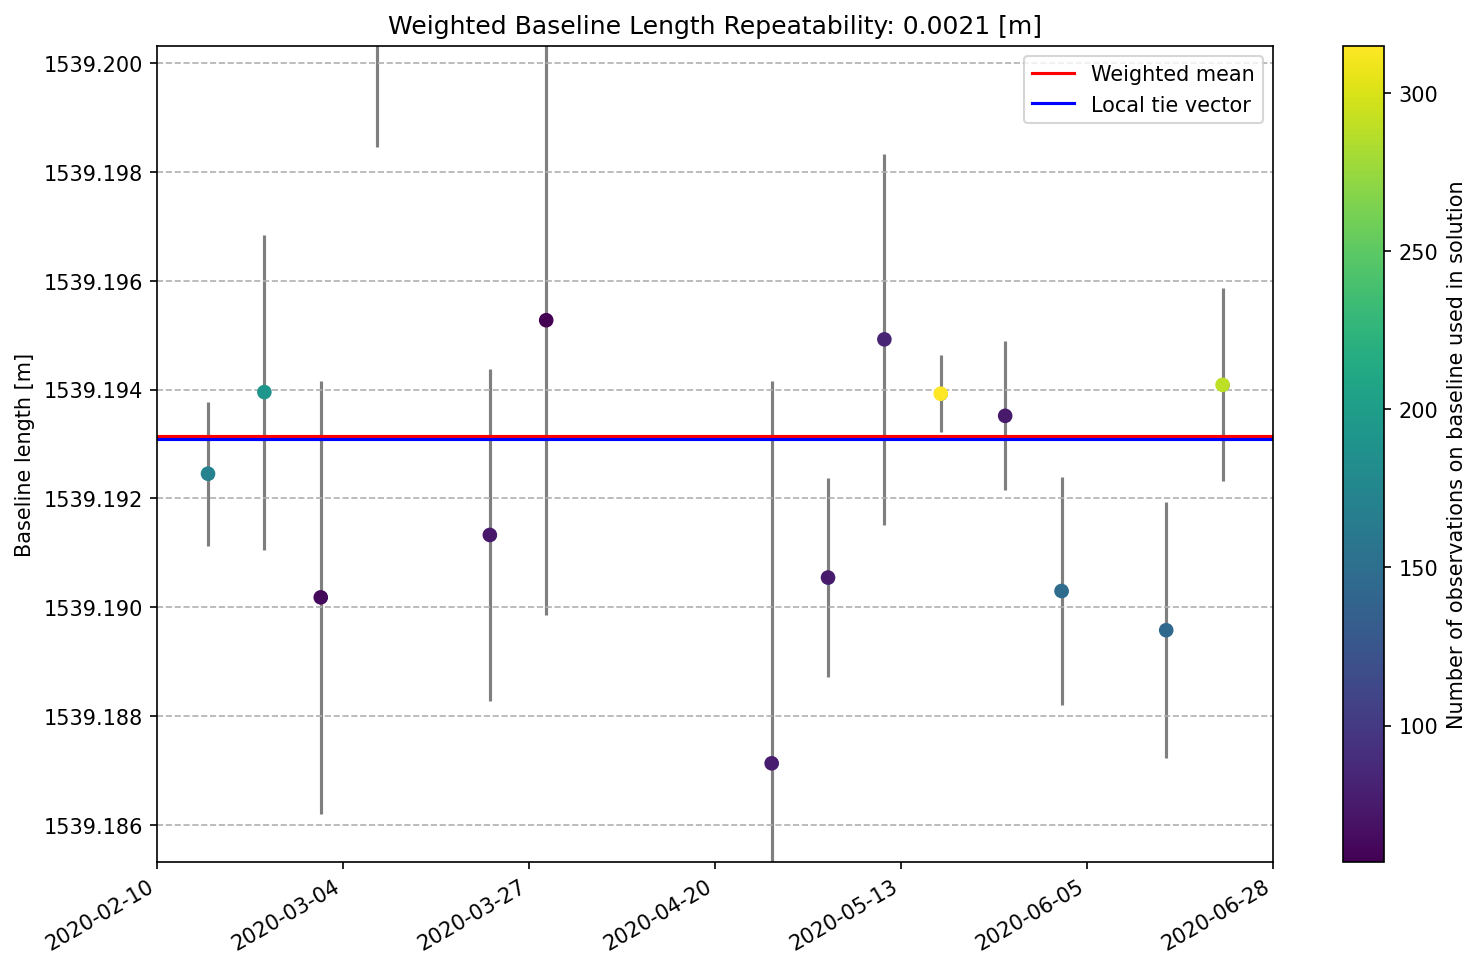
\includegraphics[width=0.5\linewidth]{figure/Baseline_NYALES20_NYALE13S_nyale13s9}} \\
    % Position NYALE13S
	\subfloat[\textcolor{black}{Estimated position - NYALE13S- Solution 0}.\label{fig:pos-Ns-0}]
      {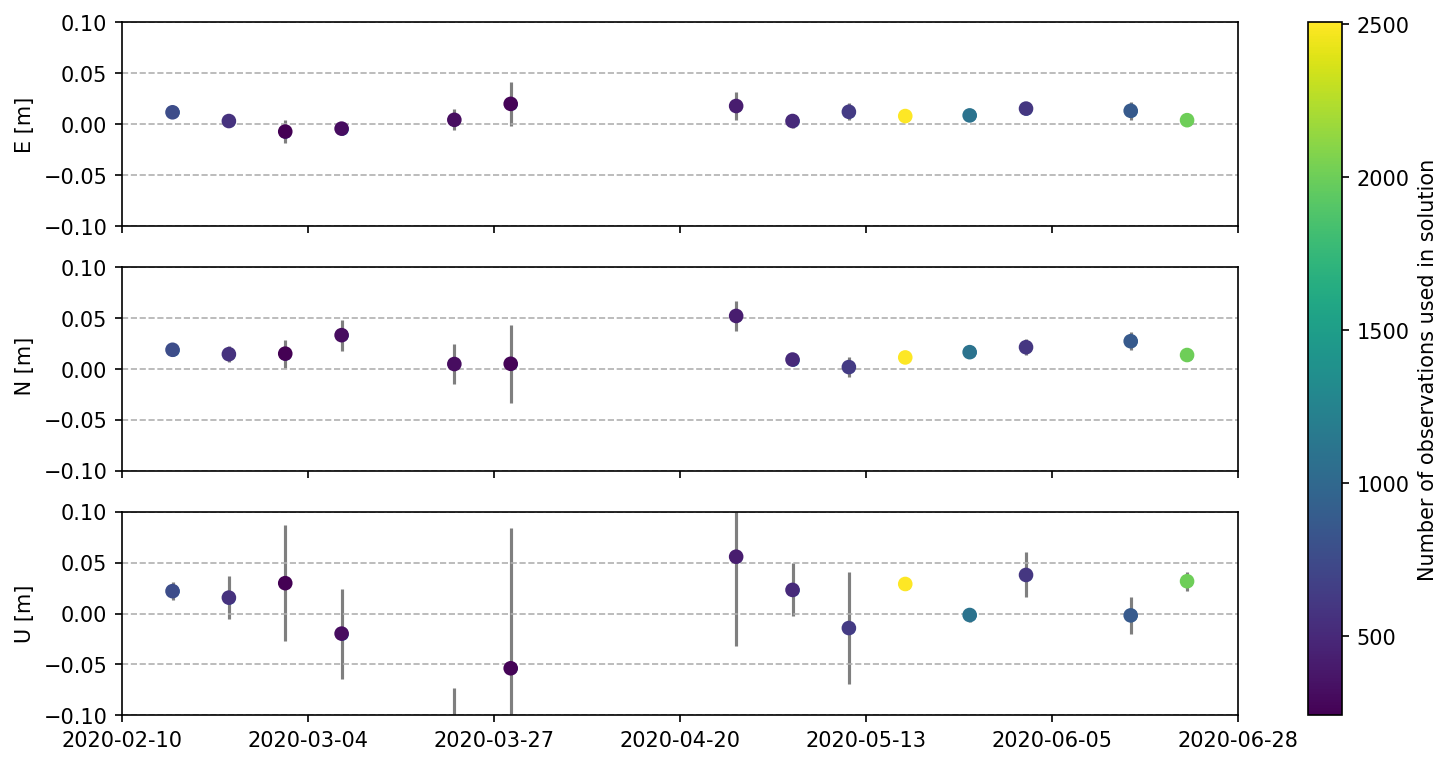
\includegraphics[width=0.5\linewidth]{figure/Position_NYALE13S_enu_nyale13s0}}
	\subfloat[\textcolor{black}{Estimated position - NYALE13S - Solution 9}.\label{fig:pos-Ns-9}]
      {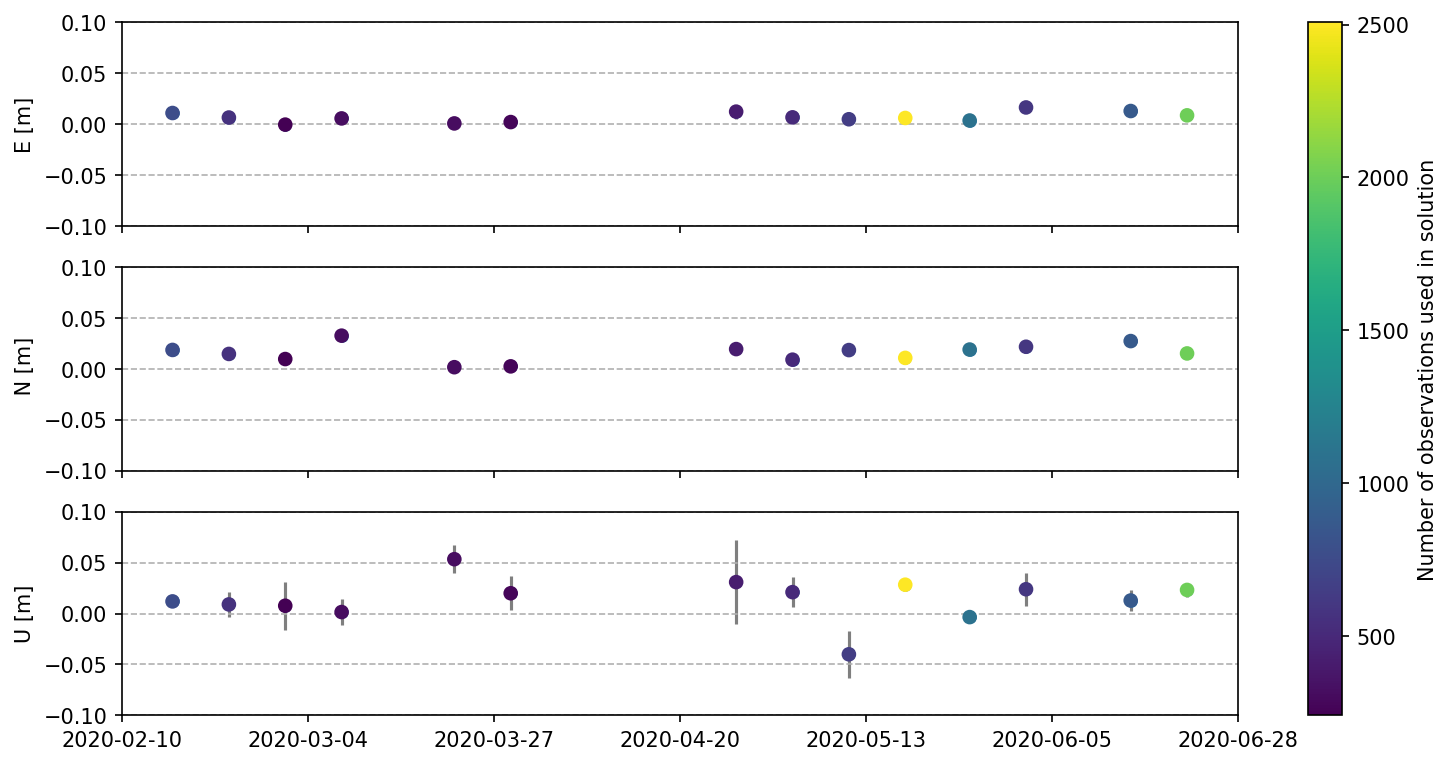
\includegraphics[width=0.5\linewidth]{figure/Position_NYALE13S_enu_nyale13s9}} \\
    % Position NYALES20
	\subfloat[\textcolor{black}{Estimated position - NYALES20 - Solution 0}.\label{fig:pos-Ny-0}]
      {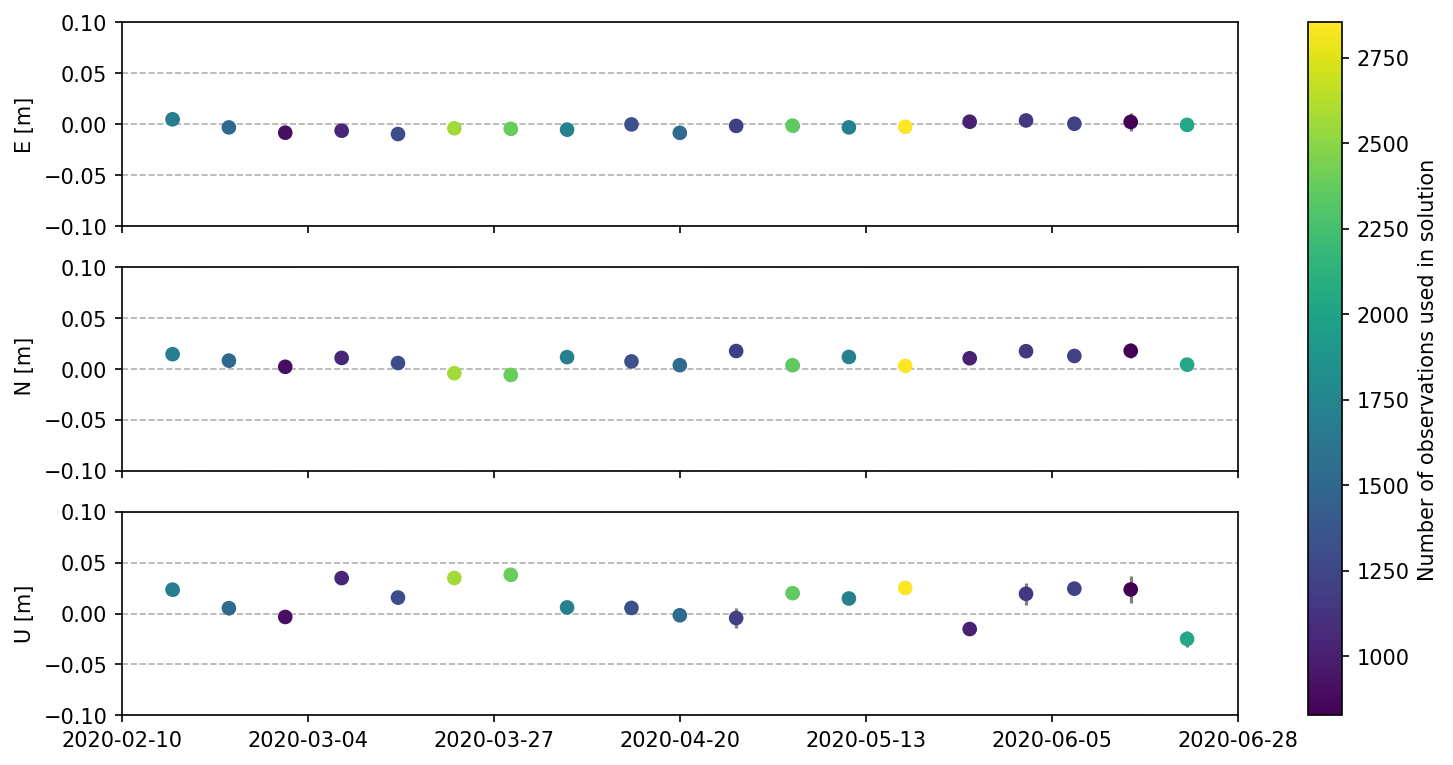
\includegraphics[width=0.5\linewidth]{figure/Position_NYALES20_enu_nyale13s0}}
	\subfloat[\textcolor{black}{Estimated position - NYALES20 - Solution 9}.\label{fig:pos-Ny-9}]
      {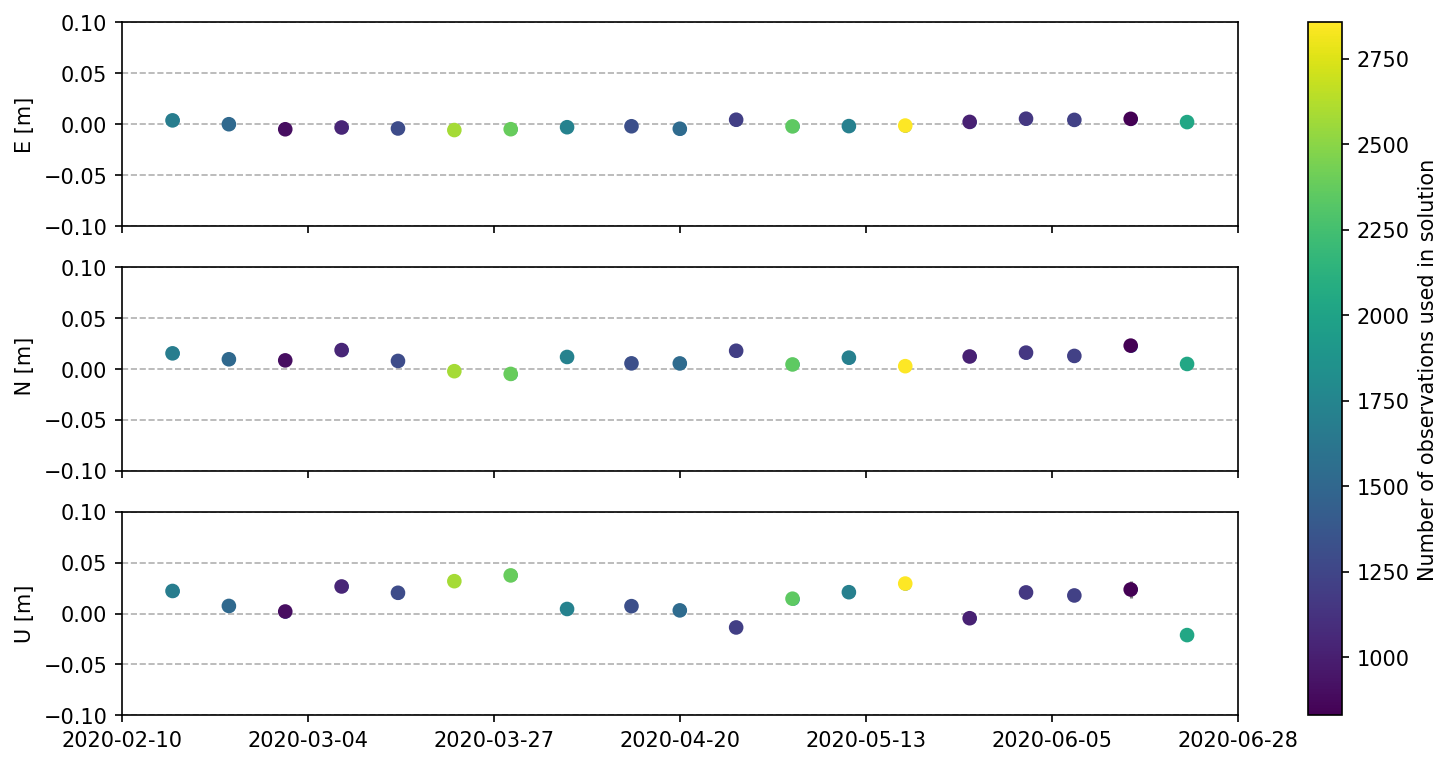
\includegraphics[width=0.5\linewidth]{figure/Position_NYALES20_enu_nyale13s9}} \\
    % RMS
	\subfloat[\textcolor{black}{Root mean square of postfit residuals [m] - Solution 0}.\label{fig:rms-0}]
      {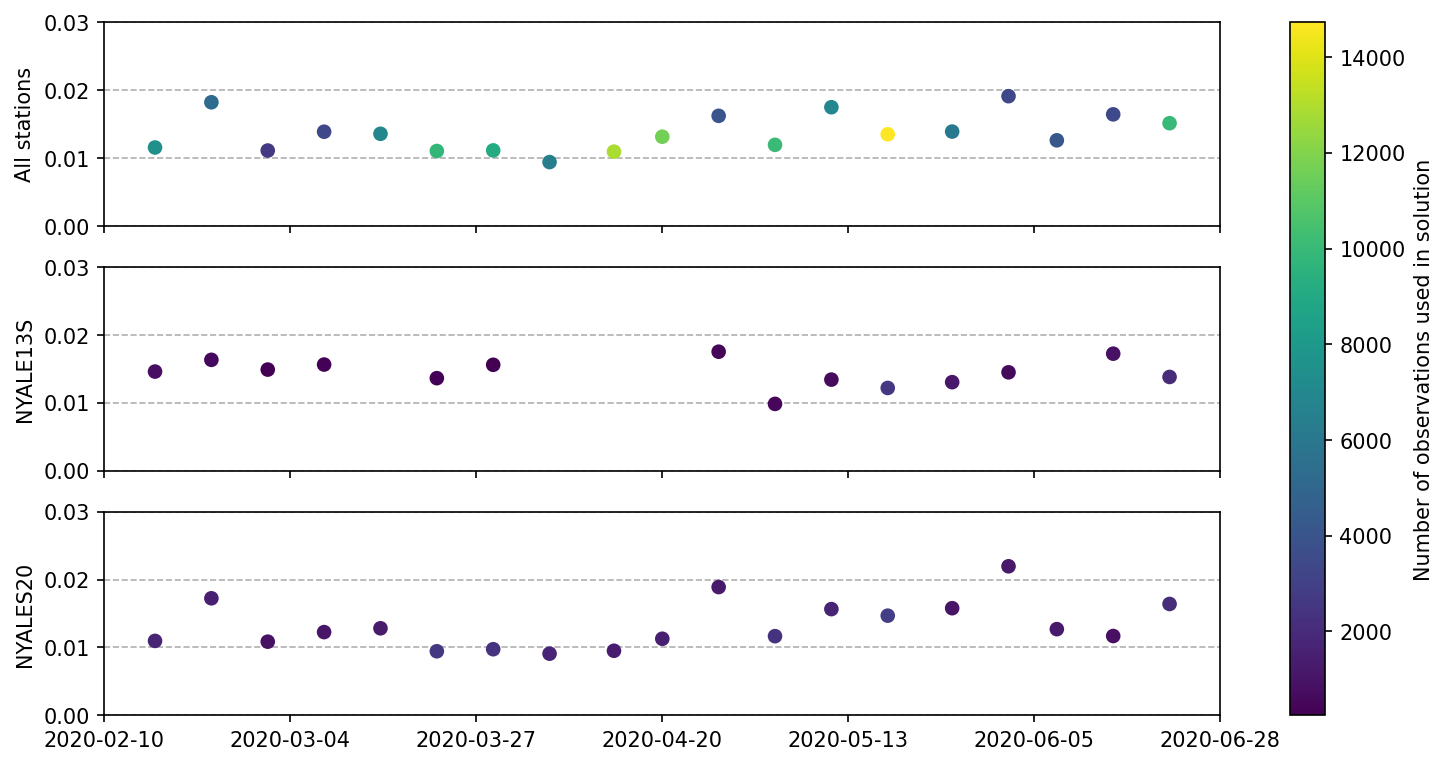
\includegraphics[width=0.5\linewidth]{figure/RMS_Postfit_Residuals_nyale13s0}}
	\subfloat[\textcolor{black}{Root mean square of postfit residuals [m] - Solution 9}.\label{fig:rms-9}]
      {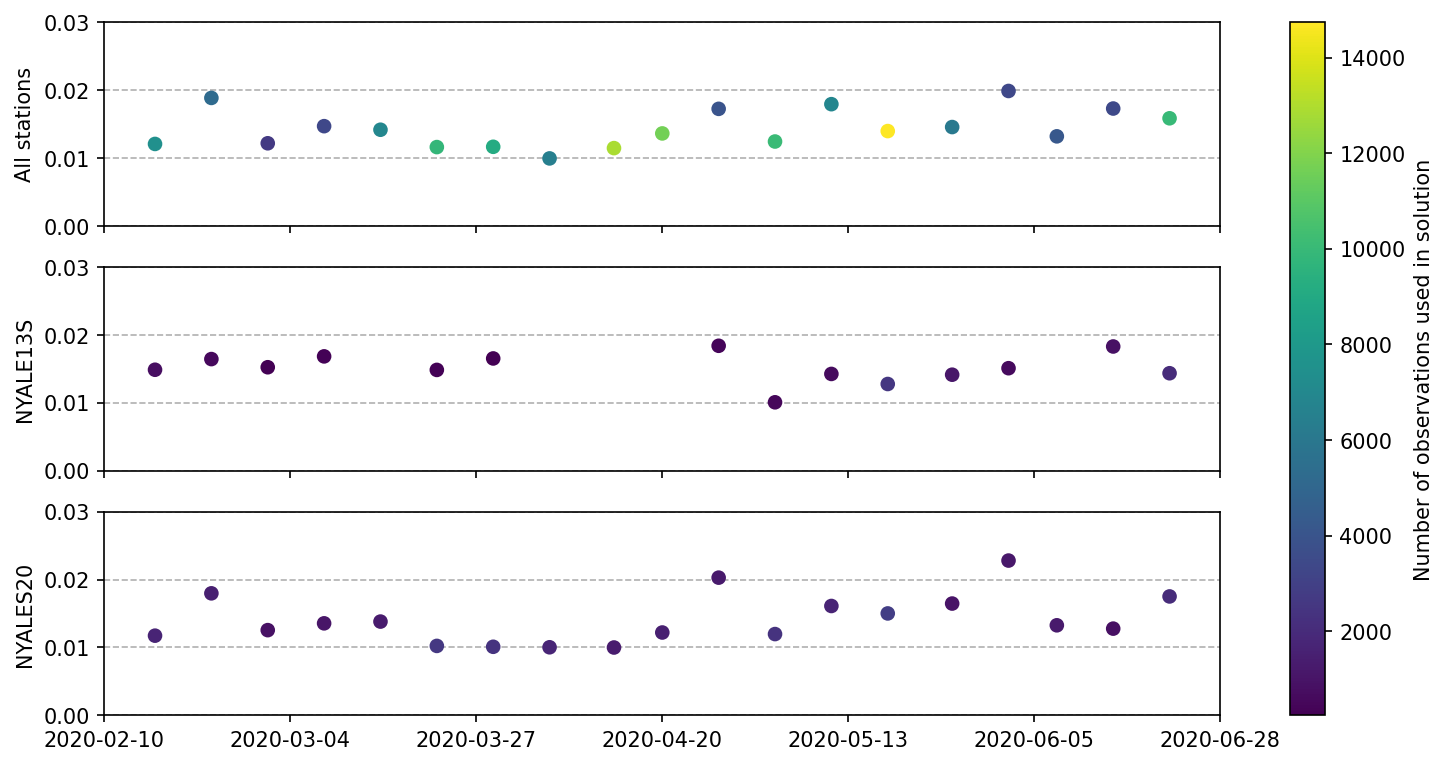
\includegraphics[width=0.5\linewidth]{figure/RMS_Postfit_Residuals_nyale13s9}} \\
    % Statistics
	\subfloat[\textcolor{black}{Statistics - Solution 0}.\label{fig:stat-0}]
      {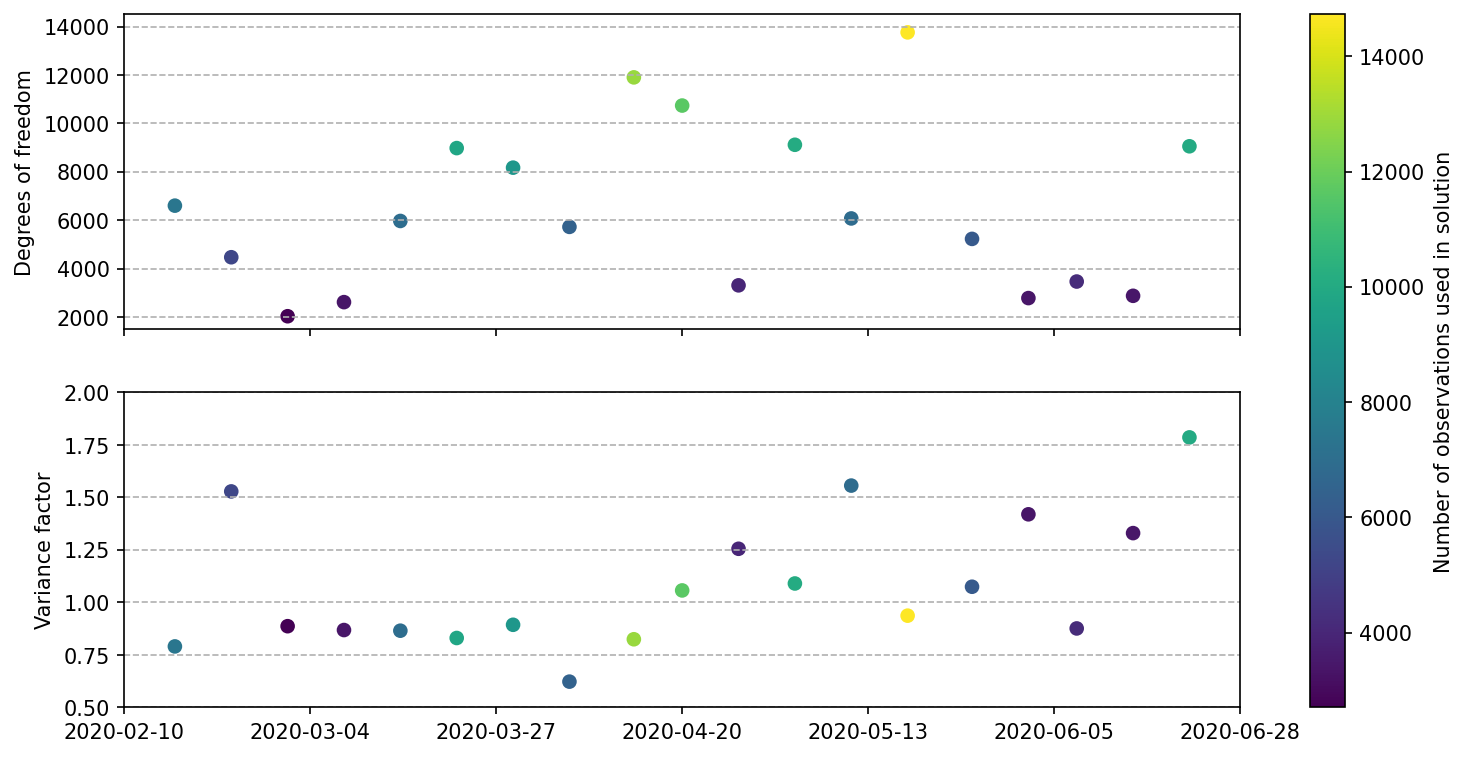
\includegraphics[width=0.5\linewidth]{figure/Statistics_nyale13s0}}
	\subfloat[\textcolor{black}{Statistics - Solution 9}.\label{fig:stat-9}]
      {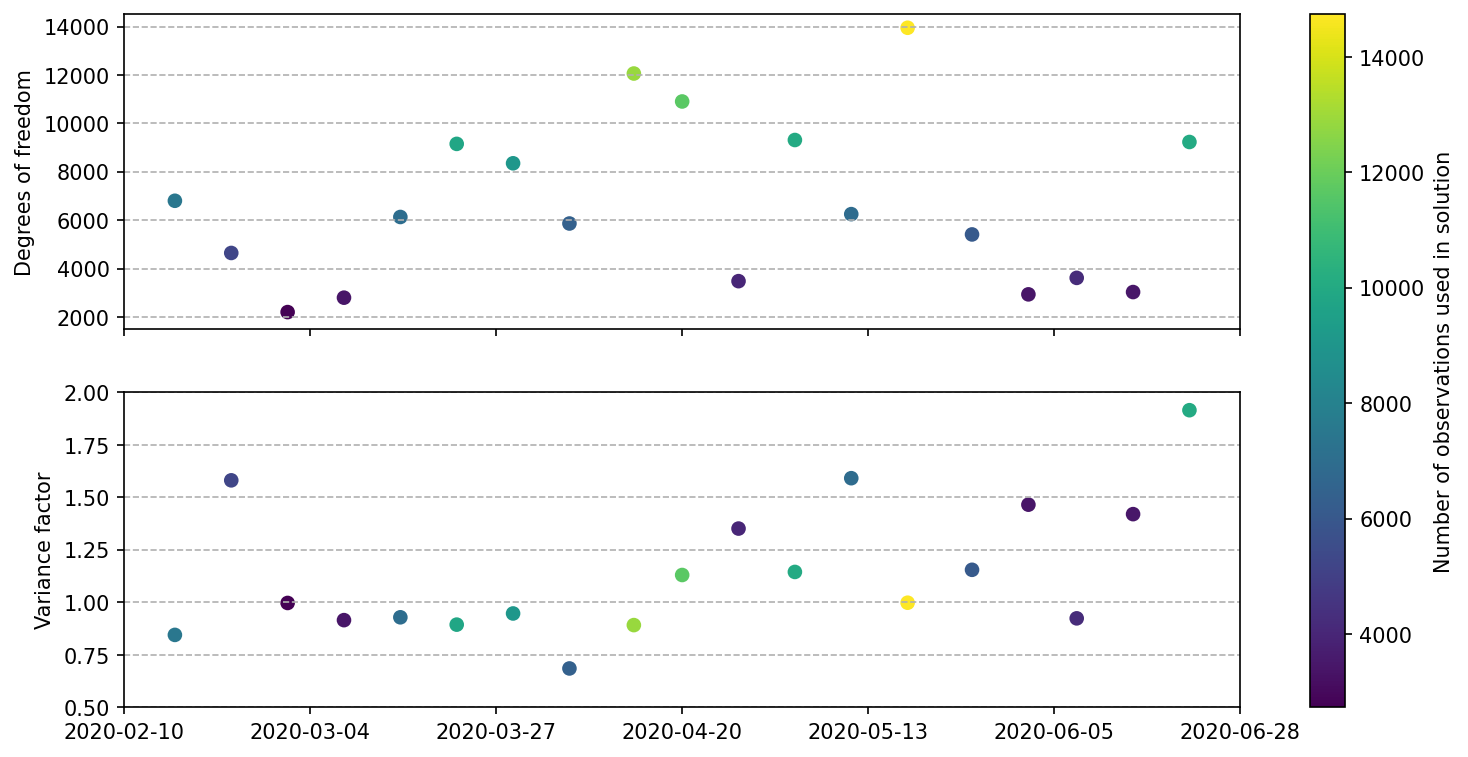
\includegraphics[width=0.5\linewidth]{figure/Statistics_nyale13s9}} \\
    %  
	\caption{Number of observations, estimated baseline length and positions for each session in addition to
	the postfit residuals and statistics for the sessions. The first column shows solution 0 and the second 
	solumn shows solution 9.}
	\label{fig:plots}
\end{figure}

\endinput

    \end{column}
    
  \end{columns}


  % References box
  \vspace*{1cm}
  \begin{columns}
    \begin{column}[t]{.15\textwidth}
      % Spacing (for Kartverket logo)
    \end{column}
    
    \begin{column}[t]{.85\textwidth}
      \begin{block}{References}
        \vspace*{-1cm}                   % Too much space on top inside block
        \begin{minipage}{.98\textwidth}  % Add space left and right
          \begin{multicols}{4}
            \footnotesize
\bibliographystyle{../../where}
\bibliography{../../where}
\endinput

          \end{multicols}
        \end{minipage}
      \end{block}
    \end{column}
  \end{columns}
\end{frame}
\end{document}
